\subsection{Experimental Setup}

Our \gls{grasp} algorithm is implemented in C++20, leveraging modern language features for efficient memory management and performance.
The implementation uses the Boost libraries for data structures and the Gurobi optimization suite (Gurobi Optimizer version 12.0.2 build v12.0.2rc0 (ARM64 - Darwin 24.5.0 24F74)) for solving the problems associated with the MIP-based heuristics.

All computational experiments were conducted on a machine equipped with an Apple M1 Pro processor running macOS 24.5.0 and an ARM64 architecture with 16GB of RAM.
The complete implementation, along with all instances used in our experiments, is publicly available at \url{https://github.com/jsalvasoler/trigger_arc_tsp}.

\subsection{Metrics}

To evaluate the performance of our \gls{grasp} algorithm, we report the optimality gap, which measures how close our solutions are to the best possible solutions. The gap is calculated as:

\begin{equation}
\text{Gap} = \frac{\text{Solution Cost} - \text{Best Known Cost}}{\text{Best Known Cost}} \times 100\%
\end{equation}

For the competition instances (C1 and C2), we use the best solutions achieved during the competition as the reference point.
For the synthetic instances (RG), we use the best integer solution obtained after running the Gurobi MIP solver for one minute.
For the randomized construction heuristics, we also measure the success rate, i.e., the percentage of instances for which a solution was found.

\subsection{Benchmarking the MIP model for the \gls{tatsp}}

We use the Gurobi solver~\cite{gurobi} to solve the MIP model defined in~\ref{sec:mip_model}.
The competition instances are significantly harder than the RG dataset, as shown in the Dataset report. In the context of MIP modeling, this is reflected in the fact
that Gurobi can only solve 6 / 21 instances of the C1 dataset, and 1 / 34 instances of the C2 dataset.
By solving, we mean that the solver was able to write the model in a reasonable time frame, and was able to provide a solution with a gap less than 1\% in under 5 hours.
For the other competition instances, the solver was not useful since it takes too long to write the model and does not provide feasible solutions or good bounds in reasonable times.
In many cases, the solver was running out of CPU memory.

Therefore, we only report the Gurobi results for the RG dataset, in which we use a time limit of 1 minute and the default settings.

\begin{table}[h]
    \caption{Performance of Gurobi MIP solver on the RG dataset of synthetic instances. Results show average computation time and optimality gap across different scenarios and problem sizes.}
    \label{tab:gurobi_performance}
    \centering
    \begin{tabular}{lrrrr}
        \toprule
        \textbf{Scenario} & \textbf{Nodes} & \textbf{Time (s)} & \textbf{Gap (\%)} \\
        \midrule
        \multirow{4}{*}{Balanced} & 10 & $1.89 \pm 2.81$ & $0.0 \pm 0.0$ \\
        & 15 & $24.04 \pm 28.83$ & $34.3 \pm 60.4$ \\
        & 20 & $34.95 \pm 29.40$ & $57.9 \pm 76.6$ \\
        & 25 & $40.84 \pm 24.70$ & $242.4 \pm 416.8$ \\
        \midrule
        \multirow{4}{*}{Decrease} & 10 & $3.90 \pm 7.38$ & $0.0 \pm 0.0$ \\
        & 15 & $25.13 \pm 27.40$ & $41.6 \pm 77.4$ \\
        & 20 & $40.14 \pm 26.30$ & $102.9 \pm 146.2$ \\
        & 25 & $48.38 \pm 19.54$ & $252.9 \pm 300.2$ \\
        \midrule
        \multirow{4}{*}{Increase} & 10 & $3.37 \pm 7.21$ & $0.0 \pm 0.0$ \\
        & 15 & $22.99 \pm 27.08$ & $36.8 \pm 83.6$ \\
        & 20 & $36.26 \pm 30.05$ & $97.1 \pm 161.7$ \\
        & 25 & $41.51 \pm 25.37$ & $154.8 \pm 215.0$ \\
        \bottomrule
    \end{tabular}
\end{table}

The three scenarios show similar behavior: all small instances (10 nodes) are solved to optimality, while both computation time and optimality gaps increase with problem size.
The Decrease scenario exhibits slightly higher gaps and longer runtimes compared to the other scenarios.

\subsection{Randomized Greedy}
We want to explore the effect of the parameter $\alpha$ on the performance of the Randomized Greedy Construction heuristic (RGC).
We run the RGC for 10 trials on each instance and each value of $\alpha$, and take the best solution found.
Recall that $\alpha \in [0, 1]$ controls the restricted candidate list (RCL) size, i.e., the fraction of the feasible edges that are considered in the greedy step, sorted by insertion cost.
Figure~\ref{fig:alpha_vs_mean_gap_randomized_greedy} shows the expected behavior of the RGC:
increasing values of $\alpha$ lead to higher gaps (since edge insertions are more expensive on average), but higher success rates (since more edges are considered).
The plot for dataset C2 shows some variability in the success rate, but we hypothesize that this behavior would dissipate with more trials.
The figure allows us to identify $\alpha = 0.1$ as a good choice for the RGC, as it provides a good balance between gap and success rate.
We will use this value for the rest of the experiments.

\begin{figure}[h]
    \centering
    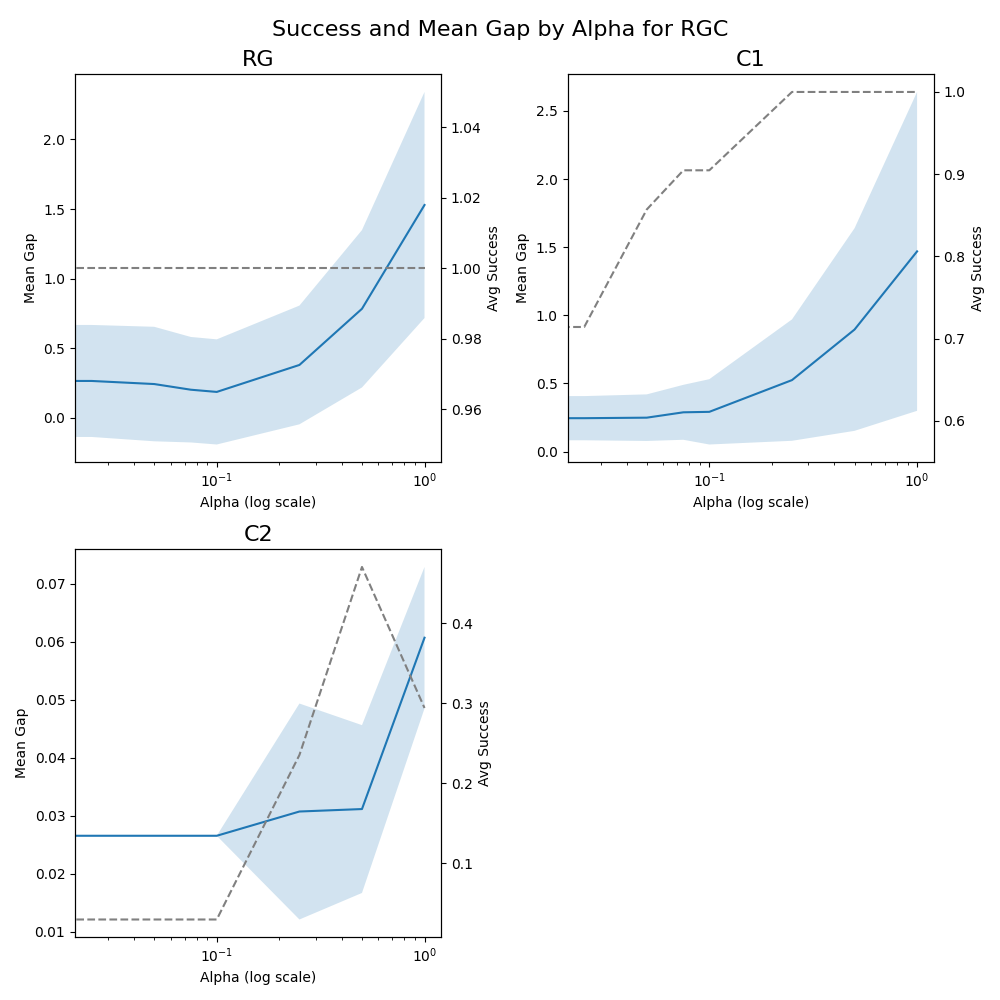
\includegraphics[width=0.49\textwidth]{figures/alpha_vs_mean_gap_randomized_greedy.png}
    \caption{Performance comparison of RGC on the three datasets. Results show average gap (\%) and success rate across different values of $\alpha$.}
    \label{fig:alpha_vs_mean_gap_randomized_greedy}
\end{figure}


\subsection{MIP Randomized Construction}

We evaluate both additive ($\gamma$) and multiplicative ($\delta$) perturbation strategies for the MIP-based random perturbation construction heuristic across different parameter values.
We set the time limit of the MIP solver to 2 seconds. Recall that solving the MIP problems to optimality is not relevant in this context, since the objective that the MIP optimizes is not
the same as the one of the \gls{tatsp}. In the context of a GRASP, exploring more initial solutions and applying local search to them is more advantageous.

\begin{table}[h]
    \caption{Performance of MIP Random Perturbation with additive noise ($\gamma$). Results show average optimality gap (\%) across different datasets and parameter values.}
    \label{tab:mip_gamma_results}
    \centering
    \setlength{\tabcolsep}{4pt}
    \begin{tabular}{lcccc}
        \toprule
        \textbf{Set} & \boldmath{$\gamma = 0.0$} & \boldmath{$\gamma = 0.1$} & \boldmath{$\gamma = 1.0$} & \boldmath{$\gamma = 10.0$} \\
        \midrule
        RG & $81.7 \pm 82.7$ & $70.9 \pm 75.6$ & $70.6 \pm 76.9$ & $\mathbf{68.9 \pm 75.3}$ \\
        C1 & $5.5 \pm 4.1$ & $\mathbf{4.3 \pm 3.2}$ & $7.3 \pm 3.9$ & $59.1 \pm 36.7$ \\
        C2 & $13.2 \pm 5.0$ & $\mathbf{6.6 \pm 2.2}$ & $7.0 \pm 2.4$ & $7.3 \pm 2.7$ \\
        \bottomrule
    \end{tabular}
\end{table}

The results for the additive perturbation parameter $\gamma$ show that moderate values ($\gamma = 0.1$) generally perform best across all datasets. On the RG dataset, higher values of $\gamma$ lead to better performance, with $\gamma = 10.0$ achieving the lowest gap of $68.9\%$. However, on the C1 dataset, $\gamma = 0.1$ is optimal ($4.3\%$ gap), while $\gamma = 10.0$ causes severe degradation ($59.1\%$ gap). The C2 dataset also favors $\gamma = 0.1$ ($6.6\%$ gap), with performance degrading for higher values.

\begin{table}[h]
    \caption{Performance of MIP Random Perturbation with multiplicative noise ($\delta$). Results show average optimality gap (\%) across different datasets and parameter values.}
    \label{tab:mip_delta_results}
    \centering
    \setlength{\tabcolsep}{4pt}
    \begin{tabular}{lcccc}
        \toprule
        \textbf{Set} & \boldmath{$\delta = 1.1$} & \boldmath{$\delta = 1.5$} & \boldmath{$\delta = 2.0$} & \boldmath{$\delta = 5.0$} \\
        \midrule
        RG & $\mathbf{69.1 \pm 72.8}$ & $70.7 \pm 76.0$ & $70.3 \pm 76.3$ & $69.9 \pm 74.6$ \\
        C1 & $4.9 \pm 4.2$ & $4.8 \pm 3.6$ & $\mathbf{4.3 \pm 3.2}$ & $4.4 \pm 3.9$ \\
        C2 & $6.6 \pm 2.7$ & $\mathbf{6.4 \pm 1.9}$ & $7.5 \pm 3.2$ & $6.9 \pm 2.8$ \\
        \bottomrule
    \end{tabular}
\end{table}

For the multiplicative perturbation parameter $\delta$, the results show that parameters have slightly different effects on datasets, indicating that the parameters are not very relevant, especially under such tight MIP solving time limits. The RG dataset performs best with $\delta = 1.1$ ($69.1\%$ gap), while C1 favors $\delta = 2.0$ ($4.3\%$ gap) and C2 performs best with $\delta = 1.5$ ($6.4\%$ gap). However, we will pick $\gamma = 0.1$ and $\delta = 1.5$ as the best parameters since they perform well on average across all datasets.


\subsection{MIP Biased Construction}

We evaluate the performance of the MIP-based biased construction heuristic
using the grid of values $\alpha \in [0.05, 0.1, 1.0, 3.0]$ and $\beta \in [0.05, 0.1, 1.0, 3.0]$.
Figure~\ref{fig:alpha_beta_grid_mip_randomized_construction_bias} shows the heatmap of average gaps across different $\alpha$ and $\beta$ combinations for each dataset.
The darker colors indicate better performance (lower gaps), allowing us to identify optimal parameter combinations for each dataset. 

For the RG and C1 datasets, higher values of $\alpha$ are better, while for the C2 dataset, lower values of $\beta$ are better. On all datasets, higher values of $\beta$ are better.
We will use the following parameter values for the rest of the experiments: $\alpha = 0.1$ and $\beta = 3.0$, which are a good trade-off in all datasets.

\begin{figure}[h]
    \centering
    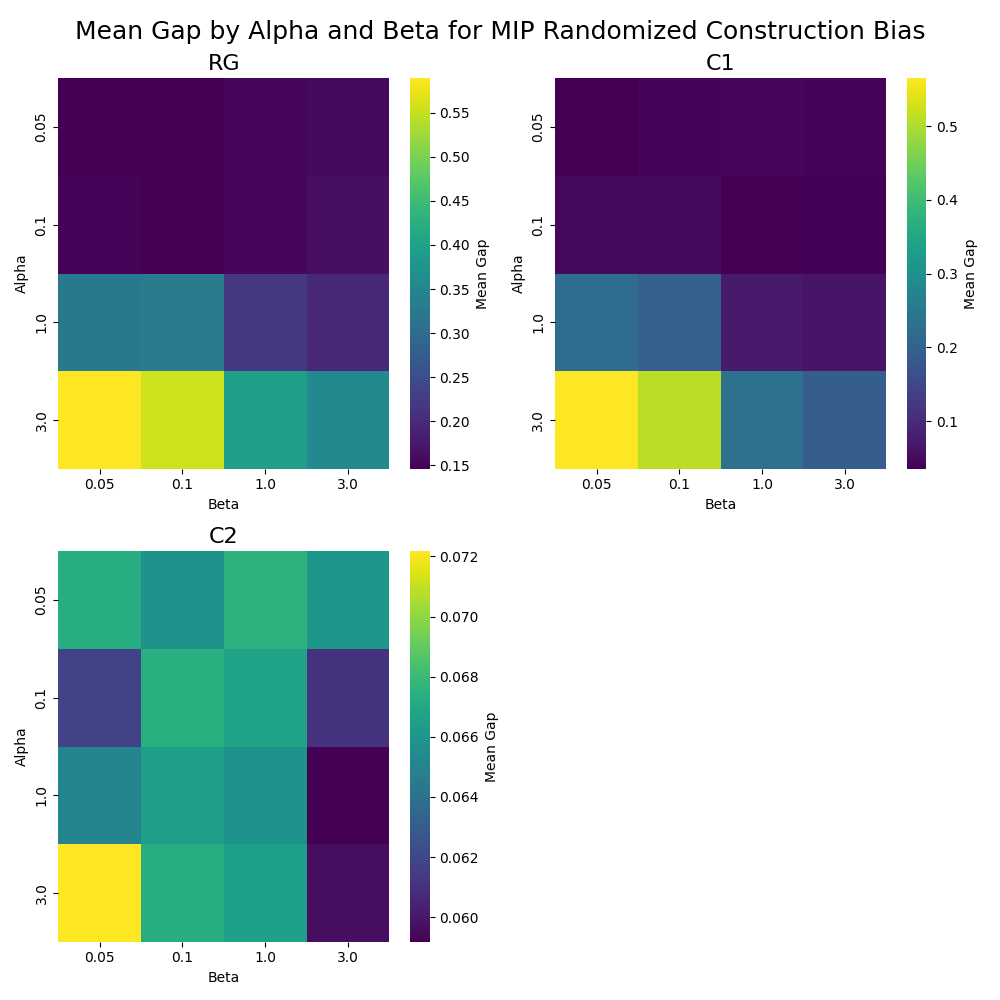
\includegraphics[width=0.49\textwidth]{figures/alpha_beta_grid_mip_randomized_construction_bias.png}
    \caption{Performance comparison of MIP Biased Construction with parameters $\alpha$ and $\beta$ on different datasets. Results show average optimality gap (\%) across different parameter combinations.}
    \label{fig:alpha_beta_grid_mip_randomized_construction_bias} 
\end{figure} 

\subsection{Comparison of Construction Heuristics}

We finally compare the performance of the tuned construction heuristics on all datasets in Table~\ref{tab:construction_comparison}.
We include another method, namely a Simple Random Construction (SRC) heuristic, in which at every step, randomly selects a feasible edge from the feasible set, without considering the insertion cost.

We find that all datasets show the same ranking pattern: MIP Bias consistently achieves the best performance, followed by MIP $\gamma$-Rand and MIP $\delta$-Rand, with RGC and SRC performing significantly worse.
The MIP-based methods demonstrate superior solution quality across all datasets, with gaps ranging from 3.8\% to 6.6\% on competition instances (C1, C2) and around 70\% on synthetic instances (RG). This suggests that leveraging a TSP solver to establish a strong underlying tour structure is highly effective, even when the costs are perturbed.
In the case of the MIP-Bias method, the perturbations successfully guide the search towards regions of the solution space that are favorable for the TA-TSP objective.
In contrast, the simpler heuristics (SRC, RGC) show much higher gaps, particularly on the RG dataset where SRC reaches nearly 300\% gap. Notably, SRC fails completely on C2 (0\% success rate), while RGC shows poor performance on C2 (2.9\% success rate).
The MIP methods maintain 100\% success rates because finding feasibility for the TSP is easy on our datasets. Runtime analysis reveals that SRC and RGC are the fastest (under 0.1 seconds), while MIP methods require 1-6 seconds, with MIP approaches taking a bit longer.
However, all methods except for Gurobi are fast enough to be used in a real-time application, which is one of our main goals.
Given these results, the construction heuristic that we will use in the GRASP framework is MIP Bias.


\begin{table}[h]
    \caption{Performance comparison of construction heuristics across all datasets. Results show average gap (\%), runtime (seconds), and success rate for each method-dataset combination.}
    \label{tab:construction_comparison}
    \centering
    \setlength{\tabcolsep}{2.1pt}
    \begin{tabular}{llrrr}
        \toprule
        \textbf{Set} & \textbf{Method} & \textbf{Gap (\%)} & \textbf{Time (s)} & \textbf{Success} \\
        \midrule
        \multirow[c]{6}{*}{C1} & SRC & $163.6 \pm 128.5$ & $0.0 \pm 0.0$ & $0.95$ \\
        & RGC ($\alpha = 0.1$) & $29.2 \pm 24.6$ & $0.1 \pm 0.1$ & $0.91$ \\
        & MIP $\gamma$-Rand(0.1) & $4.3 \pm 3.2$ & $3.2 \pm 3.7$ & $1.00$ \\
        & MIP $\delta$-Rand(1.5) & $4.8 \pm 3.7$ & $3.2 \pm 3.4$ & $1.00$ \\
        & MIP Bias(0.1, 3.0) & $\mathbf{3.8 \pm 2.8}$ & $4.1 \pm 5.2$ & $1.00$ \\
        \midrule
        \multirow[c]{6}{*}{C2} & SRC & $-$ & $0.0 \pm 0.0$ & $0.00$ \\
        & RGC ($\alpha = 0.1$) & $2.7$ & $1.5 \pm 1.7$ & $0.03$ \\
        & MIP $\gamma$-Rand(0.1) & $6.6 \pm 2.2$ & $6.1 \pm 3.8$ & $1.00$ \\
        & MIP $\delta$-Rand(1.5) & $6.4 \pm 1.9$ & $5.9 \pm 3.7$ & $1.00$ \\
        & MIP Bias(0.1, 3.0) & $\mathbf{6.1 \pm 1.8}$ & $1.9 \pm 1.5$ & $1.00$ \\
        \midrule
        \multirow[c]{6}{*}{RG} & Gurobi & $85.1 \pm 192.5$ & $26.9 \pm 27.5$ & $1.00$ \\
        & SRC & $296.4 \pm 236.0$ & $0.0 \pm 0.0$ & $1.00$ \\
        & RGC ($\alpha = 0.1$) & $66.8 \pm 59.0$ & $0.0 \pm 0.0$ & $1.00$ \\
        & MIP $\gamma$-Rand(0.1) & $70.9 \pm 75.8$ & $1.1 \pm 1.9$ & $1.00$ \\
        & MIP $\delta$-Rand(1.5) & $70.7 \pm 76.2$ & $1.1 \pm 1.9$ & $1.00$ \\
        & MIP Bias(0.1, 3.0) & $\mathbf{69.7 \pm 75.1}$ & $1.1 \pm 1.8$ & $1.00$ \\
        \bottomrule
    \end{tabular}
\end{table}

\subsection{GRASP Framework}

We now report the results of the GRASP framework. 
Based on the results of the previous section, we used the MIP Bias construction heuristic with parameters $\gamma = 0.1$ and $\delta = 3.0$.
We set a time limit of 60 seconds for the whole algorithm, and 2 seconds for the MIP solver.
We do not limit the number of trials or iterations of the GRASP. We benchmark the GRASP framework with the three local search operators: Relocate, SwapTwo, and TwoOpt.
Moreover, we ablate these operators one by one, and report the performance of the GRASP framework without each operator.


\begin{table}[h]
    \caption{Performance of GRASP framework variants across different datasets. Results show average optimality gap (\%) for different local search configurations. The smallest (best) gap in each dataset is \textbf{bolded}.}
    \label{tab:grasp_performance}
    \centering
    \begin{tabular}{llr}
        \toprule
        \textbf{Set} & \textbf{Method} & \textbf{Gap (\%)} \\
        \midrule
        \multirow[c]{4}{*}{RG} 
            & GRASP & $-11.33 \pm 26.20$ \\
            & w/o Relocate & $-8.35 \pm 24.93$ \\
            & w/o SwapTwo & $-11.56 \pm 25.75$ \\
            & w/o TwoOpt & $\mathbf{-11.59 \pm 25.80}$ \\
        \midrule
        \multirow[c]{4}{*}{C1} 
            & GRASP & $\mathbf{0.77 \pm 1.22}$ \\
            & w/o Relocate & $4.85 \pm 10.02$ \\
            & w/o SwapTwo & $1.58 \pm 3.46$ \\
            & w/o TwoOpt & $2.72 \pm 6.86$ \\
        \midrule
        \multirow[c]{4}{*}{C2} 
            & GRASP & $\mathbf{0.40 \pm 0.41}$ \\
            & w/o Relocate & $0.99 \pm 0.74$ \\
            & w/o SwapTwo & $0.50 \pm 0.45$ \\
            & w/o TwoOpt & $\mathbf{0.40 \pm 0.35}$ \\
        \bottomrule
    \end{tabular}
\end{table}

The results show that the different local search operators have varying effects across datasets.
The ablation results clearly indicate that using all three local search operators—Relocate, SwapTwo, and TwoOpt—simultaneously yields the best overall performance.
The Relocate operator is particularly important on all datasets, since removing it leads to a significant increase in the gap.

In general, the proposed GRASP framework shows to be very effective to provide fast and good solutions for the \gls{tatsp}.
The negative gaps on the RG dataset demonstrate that even on small instances, GRASP is more effective than the Gurobi MIP solver when both are operating on short time limits (60 seconds).
On the C1 and C2 datasets, the GRASP framework is able to provide final mean gaps of 0.77\% and 0.40\% respectively, which is an excellent performance for a heuristic running in a 1-minute time budget.

\paragraph{GRASP settings for the MESS 2024 competition}

We used the full GRASP with the MIP Bias construction heuristic with parameters $\gamma = 0.1$ and $\delta = 3.0$.
We used the Relocate, SwapTwo, and TwoOpt local search operators, as suggested by the ablation results.
We set the time limit of the MIP solver to 5 seconds, and the time limit of the GRASP to 3 hours per instance.
Again, we did not limit the number of trials or iterations of the GRASP.

In the repository, we provide the best solutions and the final objective values for each of the competition instances.


\section{Conclusion}
In this work, we presented a fast and effective GRASP-based metaheuristic for the recently introduced Trigger Arc Traveling Salesman Problem (TA-TSP).
Our approach combines a novel MIP-based construction heuristic with a multi-neighborhood local search procedure to efficiently explore the complex, path-dependent solution space of the TA-TSP.

Computational experiments on a diverse set of benchmark instances, including those from the MESS 2024 competition, demonstrate the superiority of our method. The proposed GRASP framework consistently finds high-quality solutions, often within a one-minute time budget, achieving near-optimal results on competition instances with average gaps below 1\%. This performance significantly surpasses that of exact MIP solvers like Gurobi, which struggle to find feasible solutions or provide useful bounds for large-scale instances within practical time limits, highlighting the necessity of metaheuristic approaches for this problem.

Future research could extend this work by exploring more sophisticated local search neighborhood structures tailored to the unique trigger-target dynamics of the TA-TSP. Furthermore, a more extensive hyperparameter tuning process, potentially using automated algorithm configuration tools, could further enhance the robustness and performance of the proposed GRASP algorithm.
